\subsection{Slučaj upotrebe: Kreiranje scenarija}

\subsubsection*{Kratak opis}

Scenarista kreira scenario za animirani film i razrađuje ga u scene i šalje reditelju na odobravanje. Time nastaje prva verzija scenarija.

\subsubsection*{Akteri}
\begin{itemize}
    \item \textbf{Scenarista} -- kreira scenario i razrađuje ga u scene.
    
\end{itemize}

\subsubsection*{Preduslovi}
\begin{itemize}
    \item Scenarista je prijavljen na sistem i angažovan na projektu.
    \item Projekat animiranog filma postoji u sistemu.
\end{itemize}

\subsubsection*{Postuslovi}

\begin{itemize}
    \item Scenario je sačuvan u sistemu kao verzija 1 i povezan sa projektom.
    \item Scenario sadrži bar jednu scenu i ima status ,,Poslata na odobravanje''.
    \item Reditelju je poslato obaveštenje o novom scenariju.
    
\end{itemize}

\subsubsection*{Osnovni tok}
\begin{enumerate}
    \item Scenarista bira projekat i opciju ,,Kreiraj scenario''.
    \item Sistem prikazuje formu za unos osnovnih podataka.
    \item Scenarista popunjava formu i potvrđuje unos.
    \item Sistem proverava podatke i čuva scenario kao verziju 1 sa statusom ,,U izradi''.
    \item Scenarista bira opciju ,,Dodaj scenu'' i unosi podatke o sceni.
    \item Sistem proverava podatke i dodaje scenu u aktuelnu verziju. Koraci 5 i 6 se ponavljaju dok scenarista ne unese sve scene.
    \item Scenarista bira opciju ,,Pošalji na odobravanje''.
    \item Sistem menja status verzije u ,,Poslata na odobravanje'', obaveštava reditelja i prikazuje poruku o uspešnom slanju.
\end{enumerate}

\subsubsection*{Podtokovi: /}

\subsubsection*{Alternativni tokovi}

\paragraph*{A1: Nepopunjena ili neispravna polja}
\begin{itemize}
    \item Ovaj tok se desava u koracima 4 ili 6 osnovnog toka, ako neko obavezno polje nije popunjeno, sistem ga označava i vraća scenaristu na unos.
   \item Scenarista ispravlja podatke.
    \item Povratak na korak 3 osnovnog toka (ako se tok desio u koraku 4), odnosno na korak 5 (ako se tok desio u koraku 6).
\end{itemize}

\paragraph*{A2: Scenario već postoji}
\begin{itemize}
    \item U koraku 1 osnovnog toka, ako projekat već ima scenario. 
    \item Sistem obaveštava scenaristu da scenario već postoji i da se on menja kroz slučaj upotrebe ,,Izmena scenarija''.
    \item Slučaj upotrebe se završava.
\end{itemize}

\paragraph*{A3: Scenario nema nijednu scenu}
\begin{itemize}
    \item Ovaj tok se dešava u koraku 7 osnovnog toka, ako scenarista nije uneo nijednu scenu.
    \item Sistem ne dozvoljava slanje i obaveštava scenaristu da mora da doda bar jednu scenu.
    \item Povratak na korak 5 osnovnog toka.
\end{itemize}

\subsubsection*{Specijalni zahtevi}
\begin{itemize}
    \item Sistem beleži autora i datum kreiranja svake verzije.
\end{itemize}


\subsubsection*{Dodatne informacije}
\begin{itemize}
    \item Osnovni podaci o scenariju (koraci 2 i 3): naslov, žanr, kratak sinopsis i ciljno trajanje filma.
    \item Podaci o sceni (koraci 5 i 6): redni broj, naziv, opis radnje, lokacija, likovi koji učestvuju, dijalozi i okvirno trajanje.
    \item Status verzije: ,,U izradi'' (posle koraka 4) i ,,Poslata na odobravanje'' (posle koraka 8).
    \item Izmena scenarija, pregled istorije verzija, vraćanje na prethodnu verziju i odobravanje scenarija od strane reditelja opisani su u slučaju upotrebe ,,Izmena scenarija''.
\end{itemize}

\begin{figure}[H]
	\centering
	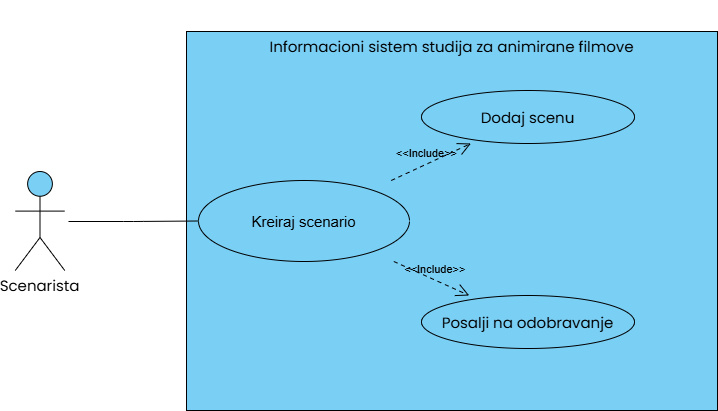
\includegraphics[width=\textwidth]{./dijagrami/dijagrami_slucajeva_upotrebe/kreiranje_scenarija.png}
	\caption{Dijagram slučaja upotrebe ,,Kreiranje scenarija''}
 \end{figure}

\begin{figure}[H]
	\centering
	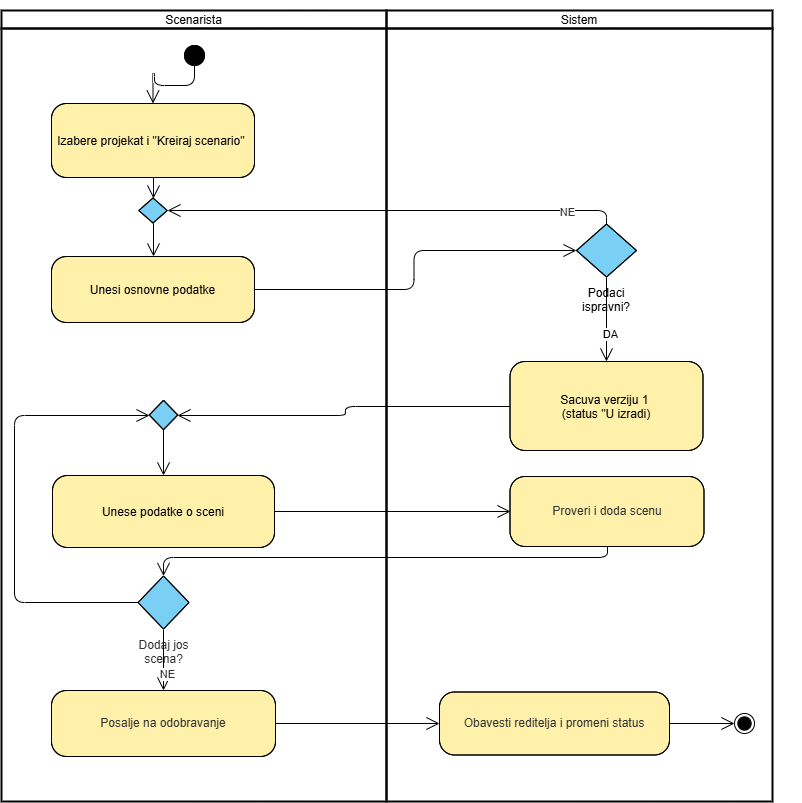
\includegraphics[width=\textwidth]{./dijagrami/dijagrami_aktivnosti/kreiranje_scenarija.png}
	\caption{Dijagram aktivnosti ,,Kreiranje scenarija''}
 \end{figure}

\begin{figure}[H]
	\centering
	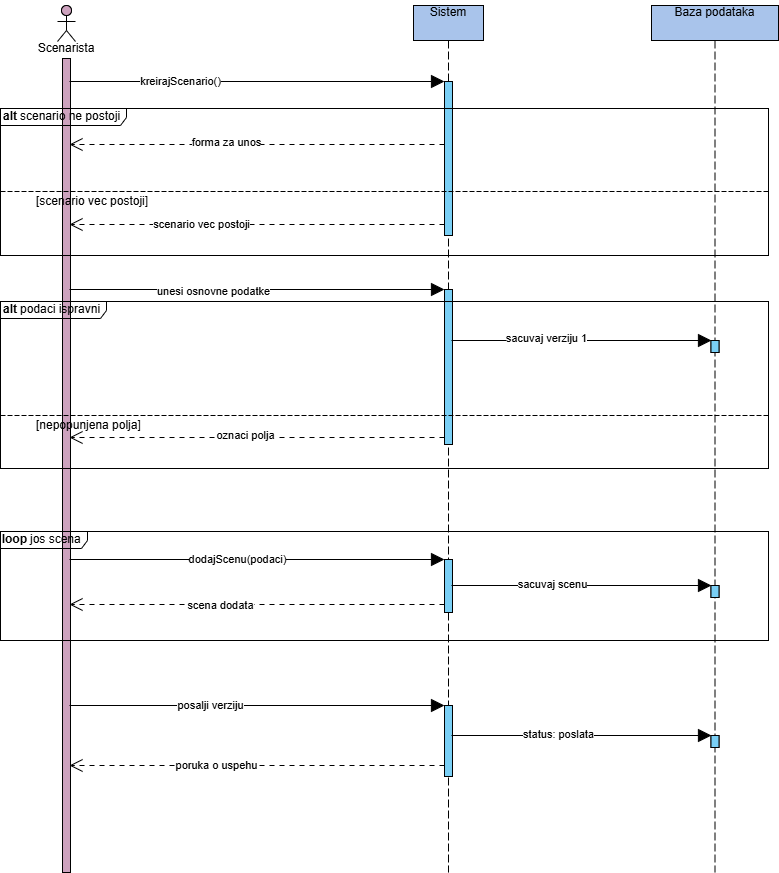
\includegraphics[width=\textwidth]{./dijagrami/dijagrami_sekvence/kreiranje_scenarija.png}
	\caption{Dijagram sekvence ,,Kreiranje scenarija''}
 \end{figure}

\newpage